\section{Use cases and validation}
\label{sec:forge:use-cases}

\subsection{Public examples}
\label{sec:forge:use-cases:golden-path}

We ran the CMS emulator example from Section~\ref{sec:methods:implementation:workflow} in Xsim and Verilator. On all six links, the decoded fields of all 217 output muons matched the CMS emulator export event by event. This checks the payload's conversion between two link-word formats.

We added one to every output muon's \texttt{eta} field and reran the example in Verilator. All 217 output words differed from the reference, each in \texttt{eta} alone. The first mismatch was on link \texttt{q0}:

\begin{codeblock}
q0, event 2, index 0, cycle 4: expected eta=1246, observed eta=1247 (valid, charge, pt, phi, d0, qual equal)
\end{codeblock}

\noindent Running \texttt{forge test --backend verilator --event-id 2} reproduced the mismatches for the two muons in that event, one on \texttt{q0} and one on \texttt{q5}. The archive includes the patch and the records from both runs.

For the second example, we simulated the CMS Level-1 track finder's VMRouter~\cite{L1TK_firmware_hls} without changing its RTL. \forge{} drives the input memories and reads the output memories using the HLS memory protocol. In Xsim, all 938 AllStub words and 938 ME stubs matched the emulation printouts over 100 events. The example uses Vitis HLS and Vivado~2024.1 and downloads test vectors from the track-finder project.

\subsection{The Phase-2 OMTF trigger processor}
\label{sec:forge:use-cases:omtf}

The Overlap Muon Track Finder reconstructs muon candidates where the CMS barrel and endcap muon systems overlap, from the stubs of drift tubes, cathode strip chambers, and resistive plate chambers. Its Phase-2 implementation for the Level-1 trigger~\cite{CMS_2020_L1TriggerUpgrade_TDR} targets an X2O board with a Virtex UltraScale+ VU13P and a 360\,MHz algorithm clock (nine cycles per 25\,ns bunch crossing). The processor has fixed latency. It receives 85 detector links, sends its candidates to the Global Muon Trigger on 18 output links, and uses the CMSSW OMTF emulator as its reference.

\begin{figure}[!htb]
  \centering
  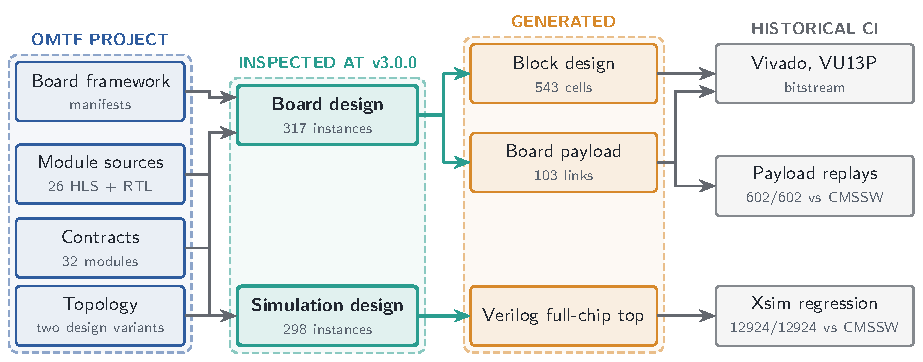
\includegraphics{figures/fig_forge_omtf}
  \caption{Board and simulation variants of OMTF. Vivado uses the board design and payload to build the bitstream. The payload replays and the full-chip Verilog regression compare outputs with the CMSSW emulator. The instance counts come from inspection with \texttt{v3.0.0}. Table~\ref{tab:forge:omtf} gives the revisions used for the CI runs.}
  \label{fig:forge:omtf}
\end{figure}

\paragraph{Design.}
The algorithm consists of 26 HLS modules, from the detector interfaces to the neural-network regression and output linking, and hand-written RTL for configuration samplers and pipeline delays. The project describes two variants (Figure~\ref{fig:forge:omtf}): the board design, with 32 modules, 317 instances, and 4357 connections, and a full-chip simulation design, with 30 modules, 298 instances, and 4038 connections, whose configuration words and output links are top-level ports instead of board-framework signals. In the board variant, all 32 modules have interface contracts. FORGE resolves the connections from 47 topology groups, 16 explicit port maps, and six contract wiring declarations without falling back to port-name matching. Both variants pass strict generation. Inspection warns that the two RPC link demultiplexers lack primary clock and reset declarations and have no exemption. The contract verifier treats these omissions as errors.

\paragraph{Latency.}
The detector branches take different numbers of cycles to reach four merge points. Using declared and HLS-reported latencies, \forge{} computes twelve delays of 2 to 73 cycles and reports all four merges as balanced. The topology requests these delays with \texttt{delay\_cycles: auto}. If resynthesis changes a module's latency, \forge{} recalculates the delays from the new reports. The board design marks 133 inputs as static, which keeps the configuration samplers out of the alignment calculation.

\paragraph{Board integration.}
The board framework supplies its ABI and endpoint manifests. \forge{} resolves the 85 input and 18 output links against them and generates the payload with the project's control policies: one register per input and output link, the replay control of the spy buffers, the lock on the bunch-crossing-zero marker, and 132 configuration words mapped to the framework's registers. The floorplan command assigns block-design cells to device regions. The project used the generated block design and payload to build a VU13P bitstream (Table~\ref{tab:forge:omtf}).

\paragraph{Verification against the emulator.}
The CI pipeline runs C simulation for 18 modules, exports the 26 HLS modules, and runs the full-chip regression. The regression matched the reference set in all 12924 output slots. A separate board-payload simulation loaded the spy buffers and replayed six sets of 100 events, one set for each processor and endcap side. All 602 muons matched the emulator in transverse momentum, pseudorapidity, and azimuth. The replay found no wrong or extra words and none outside the expected event slots.

The CI runs used earlier \forge{} revisions (Table~\ref{tab:forge:omtf}). With the same OMTF revision and HLS outputs, \texttt{v3.0.0} reproduces the Verilog tops and twelve alignment delays from \texttt{3a5bc03}, the revision used for the archived implementation.

\begin{table}[!htb]
  \centering
  \footnotesize
  \renewcommand{\arraystretch}{1.18}
  \caption{The OMTF design in \forge{}. Structure and latency from \texttt{forge inspect} and \texttt{forge dev analyze latency-check} at \texttt{v3.0.0}; the last three rows from the project's continuous integration at the commits shown.}
  \label{tab:forge:omtf}
  \begin{tabularx}{\textwidth}{@{}P{4.4cm}L@{}}
    \toprule
    Item & Value \\
    \midrule
    Board design & 32 modules, 317 instances, 4357 connections \\
    Simulation design & 30 modules, 298 instances, 4038 connections \\
    Contracts and wiring & Board variant: 32 of 32 modules have contracts, with no port-name matches \\
    Merge points; delays sized & 4, balanced; 12, from 2 to 73 cycles (both designs) \\
    Board payload & 85 input links, 18 output links, and 132 configuration words \\
    Archived VU13P implementation (\texttt{3a5bc03}) & Bitstream generated \\
    Payload replays (\texttt{03cf162}) & 6 sets of 100 events; 602 of 602 muons \\
    Regression (earlier revision) & 12924 of 12924 output slots \\
    \bottomrule
  \end{tabularx}
\end{table}

\subsection{A multi-clock image-processing pipeline}
\label{sec:forge:use-cases:vision}

The \texttt{vision\_pipeline\_demo} reference consumer contains 19 interface contracts and nine design variants, two of them invalid fixtures. Its platform-wrapper variant has 12 instances, 119 connections, and three clock and reset domains, and all 12 modules resolve through contracts. Figure~\ref{fig:forge:platform} is drawn from \forge{}'s own rendering of this design and from its archived latency report.

\begin{figure}[!htb]
  \centering
  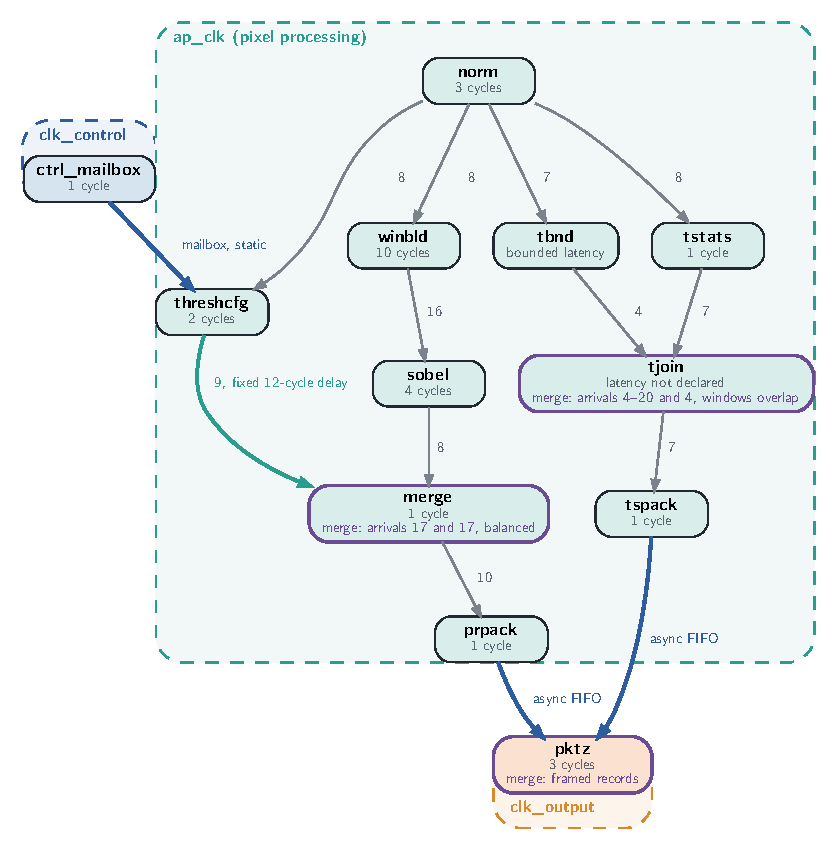
\includegraphics{figures/fig_forge_platform_wrapper}
  \caption{Platform wrapper drawn from \texttt{forge inspect --dot} and the latency report. Boxes show instances and their declared latencies. Colors group instances by clock domain. Edge labels count resolved connections, excluding clock and reset nets. Blue edges mark crossings and name their adapters. The green edge carries a fixed 12-cycle delay. Purple borders identify merges and their arrival times.}
  \label{fig:forge:platform}
\end{figure}
\FloatBarrier

The checker found no mismatches or unknown arrivals at the three merges. The pixel and threshold paths arrive at \texttt{merge} in the same cycle. At \texttt{tjoin}, the tile-boundary interval includes the statistics path's arrival (Figure~\ref{fig:forge:latency}). The packetizer takes framed records from two asynchronous FIFOs. The checker skips cycle alignment on those inputs. The threshold setting crosses domains through a mailbox. Its static declaration excludes it from alignment.

The CDC variant exercises six crossings using all four adapter kinds. In Xsim, all six checks of level status, pulse counts, and received data passed. All eight valid simulation flows passed. The scoreboard flagged an undersized FIFO with \texttt{pixel\_result\_record mismatch}. Strict generation rejected a direct bus between clock domains and reported the clock and reset domains involved.

\subsection{Validation record and reproducibility}
\label{sec:forge:results}

Table~\ref{tab:forge:results} summarizes the public results. The evidence collector reads the list of expected flows from the verification contracts. It checks complete logs for pass markers or the expected error for each invalid fixture. The trigger example includes C simulation, single-module RTL simulation, and an integrated payload test. The payload testbench waits up to 30 cycles for the output strobe and compares the response value.

\begin{table}[!htb]
  \centering
  \footnotesize
  \renewcommand{\arraystretch}{1.18}
  \caption{Results of the public examples and reference consumers, from the archived evidence. RTL simulation uses Xsim unless stated.}
  \label{tab:forge:results}
  \begin{tabularx}{\textwidth}{@{}P{4.0cm}L@{}}
    \toprule
    Item & Archived result \\
    \midrule
    CMS emulator example & 217 of 217 muons on six links, Xsim and Verilator \\
    Same, eta changed by one unit & 0 of 217 matched; every difference in eta (Verilator) \\
    VMRouter, unmodified & 938 of 938 ME and 938 of 938 AllStub words, 100 events \\
    Platform wrapper & 12 instances, 119 connections, 3 domains; 3 merges, no mismatch \\
    Vision simulations & 8 of 8 pass; both invalid fixtures rejected with their diagnostics \\
    CDC variant & 6 checks pass across the four adapter kinds \\
    Trigger consumer & 4 C-simulation, 4 single-module and 1 integrated RTL flow pass \\
    Framework test suite & 2417 passed, 12 skipped, with the EDA tools present \\
    \bottomrule
  \end{tabularx}
\end{table}

The evidence README records the tools, test skips, and packetizer measurements.

The reference-consumer logs come from one session on a clean checkout of the cited commit. The archive hashes the log files. Linking each log to the simulated executable would require per-flow build hashes. To reproduce the simulations, build and run the flows again. We ran the public example's negative control separately with Verilator~5.020.
